\section{Planung}
In diesem Dokument steht die Detailplanung für die Entwurfs- und
Realisierungssphase für die autonome Ballwurfmaschine im Zentrum.
Das Team arbeitet mit einem öffentlichen Dienst names GitHub (\href{https://github.com}{https://github.com}).
Auf GitHub wurde ein Repository (Arbeitsbereich) für das Team angelegt
(\href{https://github.com/accefa/pren2}{https://github.com/accefa/pren2}). Alle Meilensteine (milestones) und Arbeitspakete (issues) werden dort zentral verwaltet und sind immer aktuell.

\subsection{Rahmenplanung}
Das Modul PREN2 gibt gewisse Fixpunkte vor. Diese sind vom Team nicht
beeinflussbar und müssen eingehalten werden. Diese Punkte sind als
Meilensteine definiert mit dem Prefix 'Offiziell'. Ausserdem wurden weitere
Meilensteine terminiert in welchen sich das Team Zwischenziele setzt. Diese Meilensteine beginnen jeweils mit der involvierten Disziplin.

\begin{itemize}
	\item ET Elektrotechnik
	\item IT Informatik
	\item MB Maschinenbau
\end{itemize}

Auf dem Rahmenplan (siehe Abbildung \ref{fig:rahmenplanung}) ist eine grosse Lücke zwischen den letzten beiden offiziellen Meilensteinen. Wir streben das Ziel an, dass wir uns in dieser Phase nur noch um Tests und Dokumentation kümmern müssen. In den Tests können Fehler auftreten, welche in dieser Phase behoben werden müssen.

Der Terminplan ist sehr straff. Im IT und MB Bereich sehen wir keine Probleme da die Ressourcen pro Disziplin (je 3 Teammitglieder) sehr hoch sind. Der ET-Teil bereitet hier uns eher Kopfzerbrechen. Nur ein Mitglied ist aus dem ET-Bereich und dieses hat auch sehr viel Arbeit vor sich. Konsequenzen
daraus sind, dass dieses Teammitglied vollständig von jeglichen Aufgaben
entlastet wird, welches auch andere Teammitglieder erledigen können.
Dokumentieren, testen und auch Projektmanagement-Tätigkeiten müssen soweit möglich von anderen erledigt werden. Wir werden die Entwicklung der ET in den nächsten 3 Wochen genau beobachten, falls die Arbeit nicht wie geplant fortschreitet, muss gehandelt werden. Eine Massnahme wäre, dass sich ein Informatiker vollständig der Elektrotechnik widmet.

\begin{landscape}
\begin{figure}
\centering
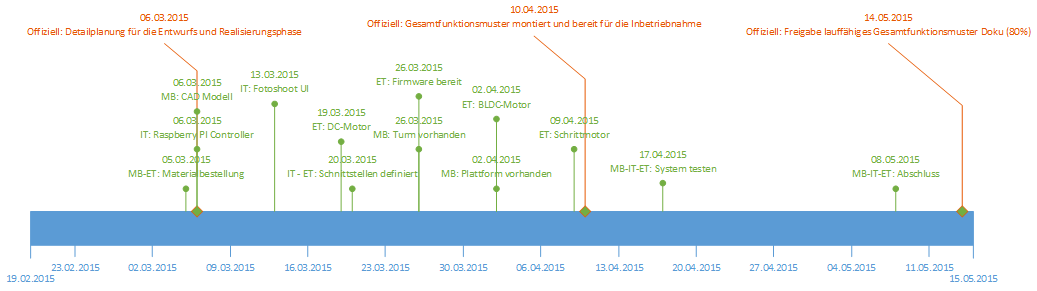
\includegraphics[width=1\linewidth]{../../fig/rahmenplanung}
\caption{Rahmenplan}
\label{fig:rahmenplanung}
\end{figure}
\end{landscape}

\subsection{Rahmenplanung (Stand: 10.04.2015)}
Am 10.04.2015 hat sich das Team zusammengeschlossen um über die restlichen Arbeiten zu diskutieren. Darauf hin hat man sich entschlossen die restliche Planung anzupassen. Nun wurden teilweise neue Termine definiert, welche für den restlichen Verlauf binden sind.

\begin{figure}[h!]
\centering
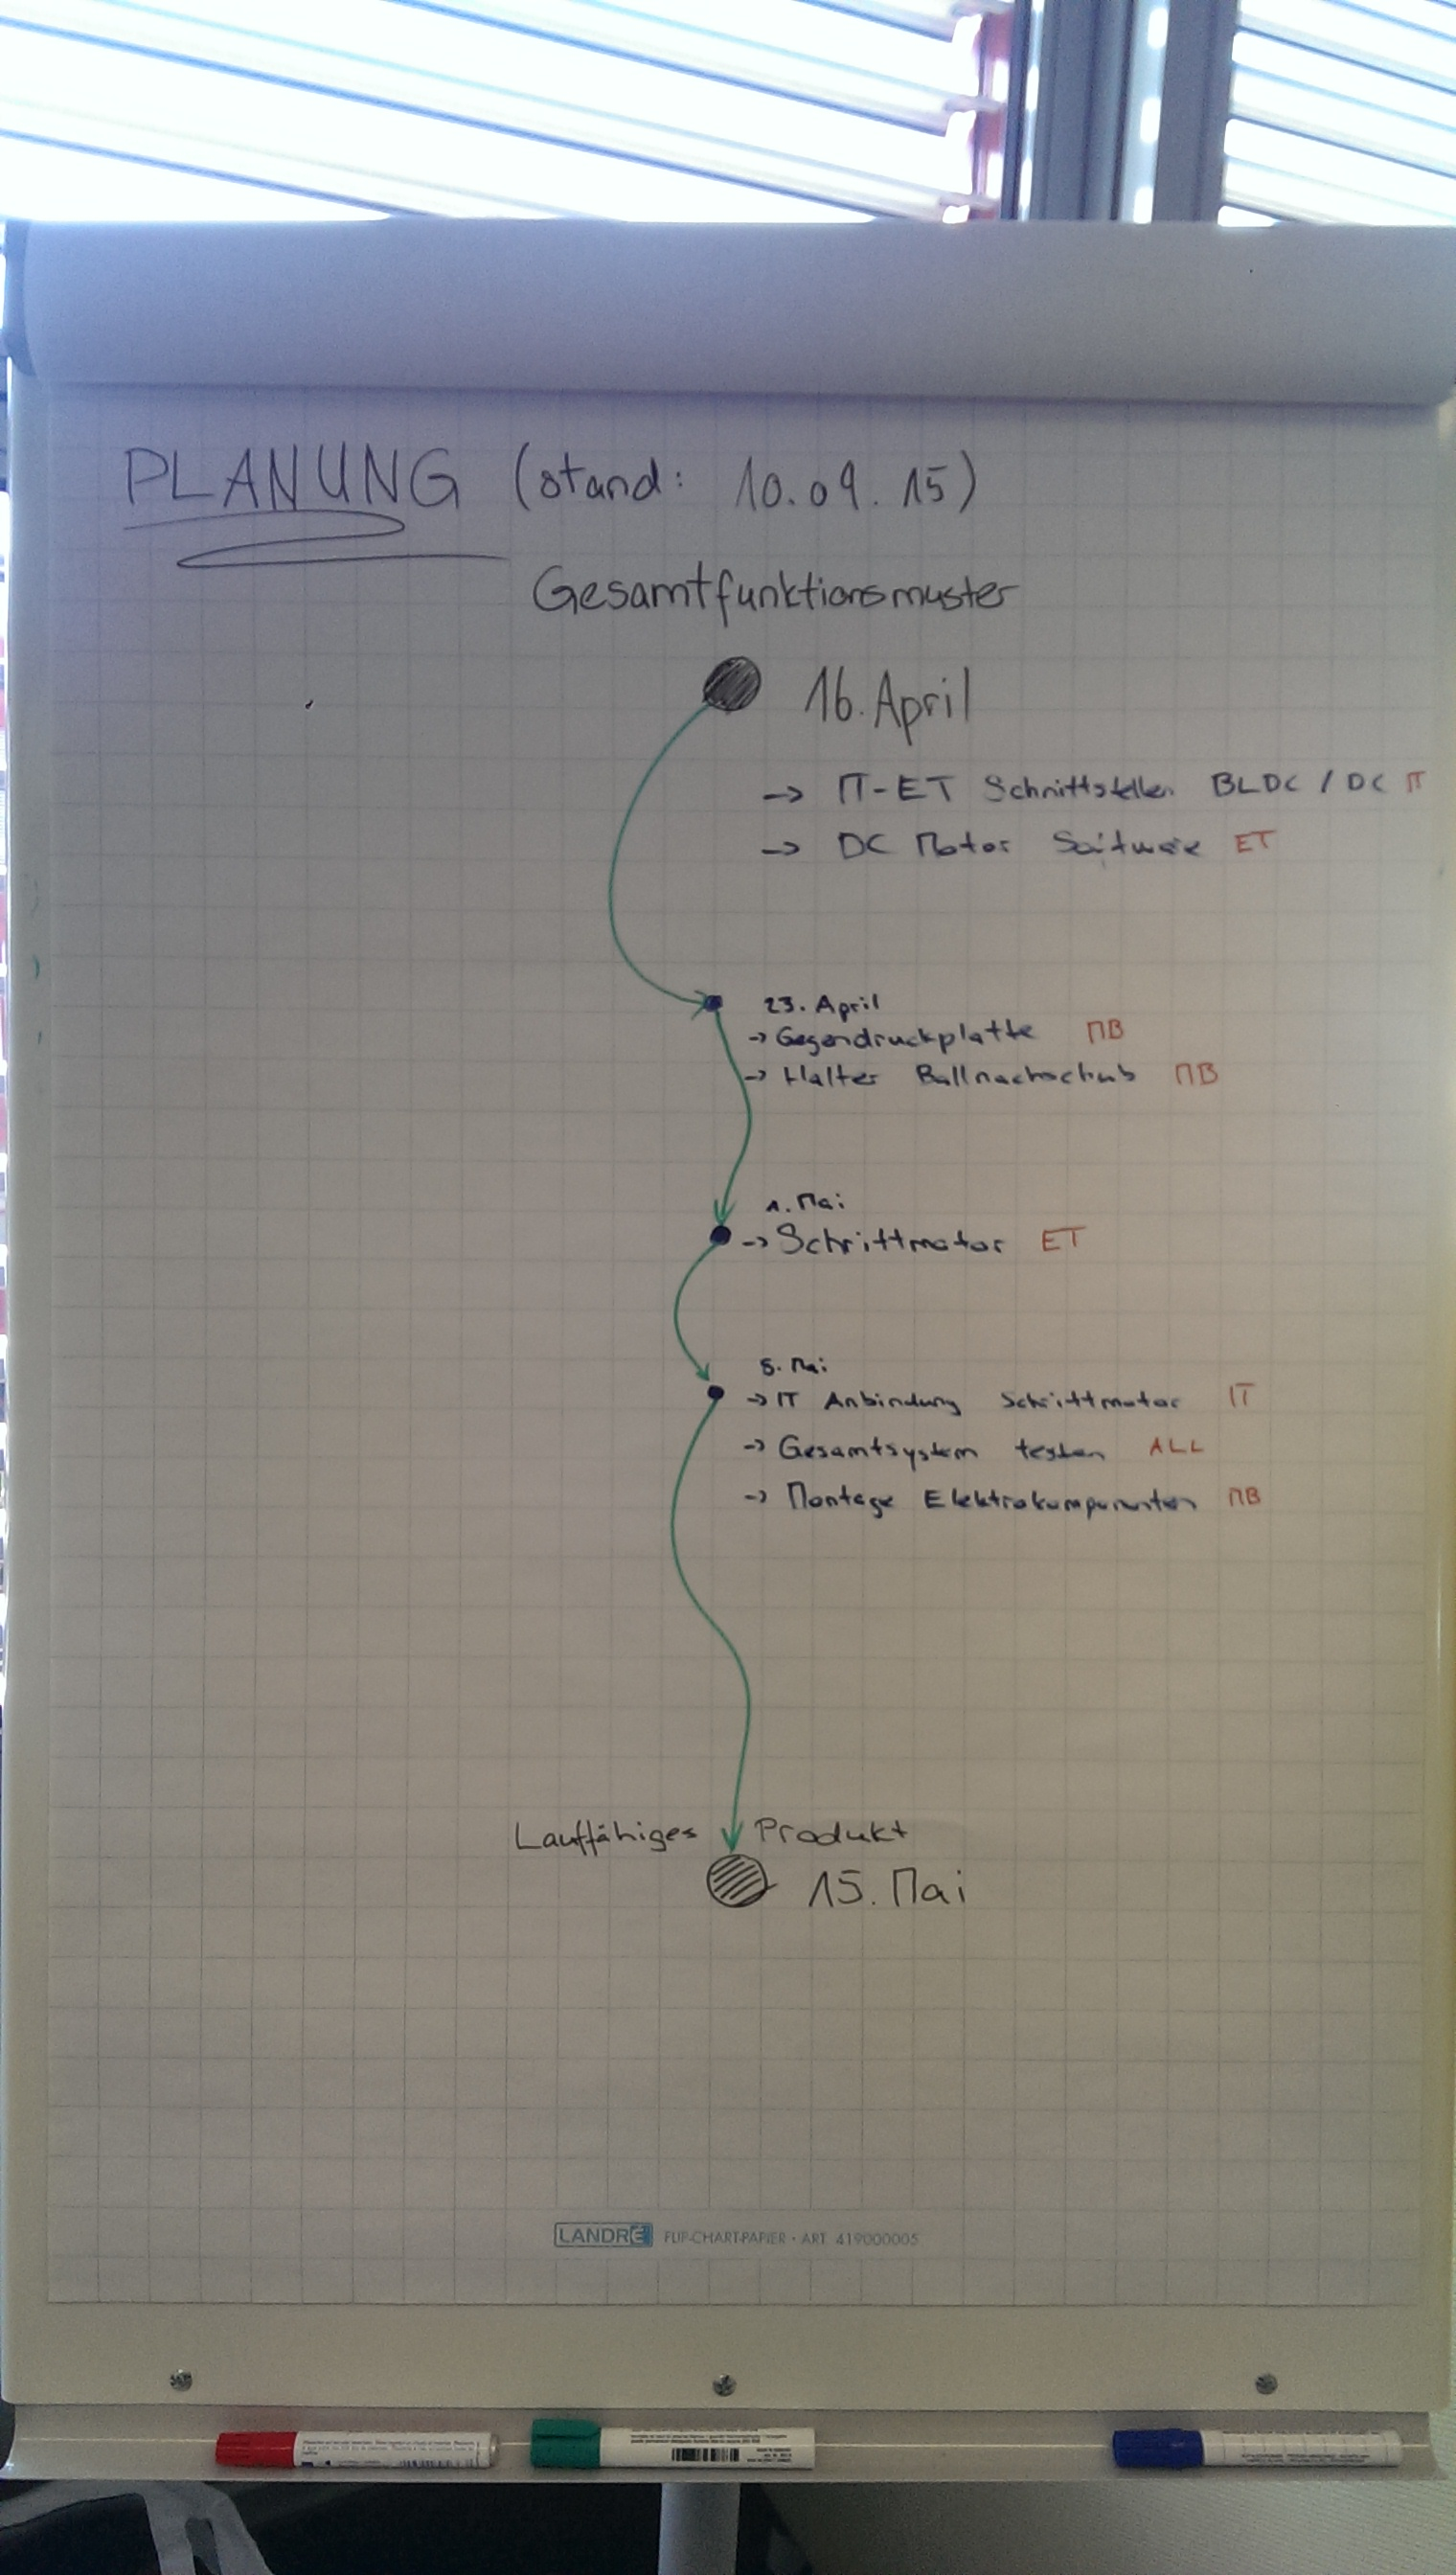
\includegraphics[width=0.6\linewidth]{../../fig/rahmenplanung-10042015}
\caption{Rahmenlanung (Stand 10.04.2015)}
\label{fig:rahmenplanung-10042015}
\end{figure}

